\documentclass[a4paper,12pt]{article}
\usepackage[brazil]{babel}
\usepackage[utf8]{inputenc}
\usepackage[T1]{fontenc}
\usepackage{geometry}
\usepackage{setspace}
\usepackage{titlesec}
\usepackage{hyperref}
\usepackage{graphicx}
\usepackage{caption}
\usepackage{subcaption}
\usepackage{fancyhdr}
\usepackage{xcolor}
\usepackage{fancyhdr}
\pagestyle{fancy}

\fancyhf{} % Limpa cabeçalhos e rodapés
\fancyhead[L]{\small Estudos -Concurso.}
\fancyhead[C]{Provas - Física}
\fancyhead[R]{Página \thepage}

%%%%%%%%%%%%%%%%%%%%%%%%%%%%%%%%%%%%%%%%%%%%%%%%%%
% These are some new commands that may be useful 
% for paper writing in general. If other new commands
% are needed for your specific paper, please feel 
% free to add here. 
%
% The currently available commands are organized in: 
% 1) Systems
% 2) Quantities
% 3) Energies and units
% 4) particle species
% 5) Colors package
% 6) hyperlink
%%%%%%%%%%%%%%%%%%%%%%%%%%%%%%%%%%%%%%%%%%%%%%%%%%

\usepackage{amsmath}
\usepackage{amssymb}
\usepackage{upgreek}
\usepackage{multirow}
\usepackage{setspace}% http://ctan.org/pkg/setspace
\usepackage{fancyhdr}
\usepackage{datetime}

% 1) SYSTEMS
\newcommand{\btc}               {\textbf{BTC}}
\newcommand{\btcspace}          {\textbf{BTC} }
\newcommand{\pow}               {\textbf{PoW}}

% 4) definition to references, biblatex and hyperlink
\usepackage[backend=bibtex, 
style=nature,  %style reference.
sorting=none,
firstinits=true %first name abbreviate
]{biblatex}

\usepackage{hyperref}
\hypersetup{
    colorlinks=true, %set "true" if you want colored links
    linktoc=all,     %set to "all" if you want both sections and subsections linked
    linkcolor=blue,  %choose some color if you want links to stand out
    citecolor= blue, % color of \cite{} in the text.
    urlcolor  = blue, % color of the link for the paper in references.
}

% 5) Tikz and figures
\usepackage{epsfig}
\usepackage{lmodern}
\usepackage{mathtools}
\usepackage[utf8]{luainputenc}
\usepackage{xspace}
\usepackage{tikz}
\usepackage{pgfplots}
\pgfplotsset{compat=newest}

\usetikzlibrary{positioning}
\usepackage{subcaption}

% 6) colors:
\usepackage{xcolor}
\definecolor{ao(english)}{rgb}{0.0, 0.5, 0.0} % dark green

% 7) Add lines numbers
%\usepackage{lineno}

% add pdf file to thesis:
\usepackage{pdfpages}

\hypersetup{
    colorlinks=true,% make the links colored
    linkcolor=blue
}

\usepackage{setspace}
\addbibresource{bibliography.bib}

\newcommand{\printingbibliography}{%

    \pagestyle{myheadings}
    \markright{}
    \sloppy
    \printbibliography[heading=bibintoc, % add to table of contents
                   title=Refer\^encias % Chapter name
                  ]
    \fussy%
}
\PassOptionsToPackage{table}{xcolor}
\renewcommand{\baselinestretch}{1.5}

\pagestyle{fancy}
\fancyhf{}
\renewcommand{\headrulewidth}{0pt}
\fancyhead[R]{\thepage}

\geometry{a4paper,top=30mm,bottom=20mm,left=30mm,right=20mm}

\titleformat*{\section}{\bfseries\large}
\titleformat*{\subsection}{\bfseries\normalsize}

\title{Resolu\c{c}\~ao de Prova de F\'isica - Inst\'itutos Federais.\\
Áreas 15 e 28 – Física – EDITAL 049/2020}
\author{Andr\'e V. Silva \\
\href{https://andrevsilva.com/}{\texttt{https://andrevsilva.com/}}}
\date{\today}

\begin{document}

\maketitle

\begin{center}
\url{https://arq.pciconcursos.com.br/provas/31060128/e7b804f2e08b/fisica.pdf}
\end{center}

\textbf{11.} \textbf{[IFSul2020 - EDITAL 049/2020]} Um automóvel encontra-se parado em um semáforo. Quando a luz verde é acesa, o automóvel parte 
com uma aceleração de $1,0 \text{ m/s}^2$ (despreze o tempo de reação do(a) motorista). Nesse instante, 
uma motocicleta encontra-se a $128$ metros atrás do automóvel, deslocando-se com velocidade constante de 
$72$ km/h na mesma direção e sentido da aceleração do automóvel. Após a motocicleta ultrapassar o automóvel, 
em quanto tempo ele tornará a ultrapassá-la?

\begin{itemize}
    \item[a)] 8 segundos.
    \item[b)] 24 segundos.
    \item[c)] 32 segundos.
    \item[d)] 40 segundos.
\end{itemize}

\section*{Resolução}

\subsection*{Passo 1: Definir as equações do movimento}

O movimento do automóvel segue a equação do \textbf{MRUV}:

\begin{equation}
    S_A = S_{0A} + v_{0A} t + \frac{1}{2} a t^2
\end{equation}
Sabemos que:
\begin{itemize}
    \item $S_{0A} = 0$
    \item $v_{0A} = 0$ (pois parte do repouso)
    \item $a = 1,0 \text{ m/s}^2$
\end{itemize}
Portanto, a equação do automóvel é:
\begin{equation}
    S_A = \frac{1}{2} t^2
\end{equation}

Já a motocicleta move-se em \textbf{MRU}, cuja equação é:
\begin{equation}
    S_M = S_{0M} + v t
\end{equation}
Sabemos que:
\begin{itemize}
    \item $S_{0M} = -128$ m (pois está atrás do automóvel)
    \item $v = 72$ km/h = $20$ m/s (convertendo: $72 \div 3.6$)
\end{itemize}
Portanto, a equação da motocicleta é:
\begin{equation}
    S_M = -128 + 20t
\end{equation}

\subsection*{Passo 2: Determinar o primeiro encontro}

Quando os dois veículos estiverem na mesma posição:
\begin{equation}
    \frac{1}{2} t^2 = -128 + 20t
\end{equation}
Multiplicando por 2 para eliminar a fração:
\begin{equation}
    t^2 - 40t + 256 = 0
\end{equation}
Resolvendo a equação quadrática por Bhaskara:
\begin{align*}
    \Delta &= (-40)^2 - 4(1)(256) = 1600 - 1024 = 576 \\
    \sqrt{576} &= 24 \\
    t &= \frac{40 \pm 24}{2}
\end{align*}
As soluções são:
\begin{align*}
    t_1 &= \frac{40 + 24}{2} = \frac{64}{2} = 32s \\ 
    t_2 &= \frac{40 - 24}{2} = \frac{16}{2} = 8s
\end{align*}
Portanto, a primeira ultrapassagem ocorre em $t = 8$ segundos.

\subsection*{Passo 3: Determinar a segunda ultrapassagem}

A segunda ultrapassagem ocorre quando o automóvel, em $t = 32$s, o tempo decorrido desde do primeiro encontro \'e 24 segundos. \fbox{Alternativa (b) 24 segundos.}


\begin{figure}[h!]
    \centering
    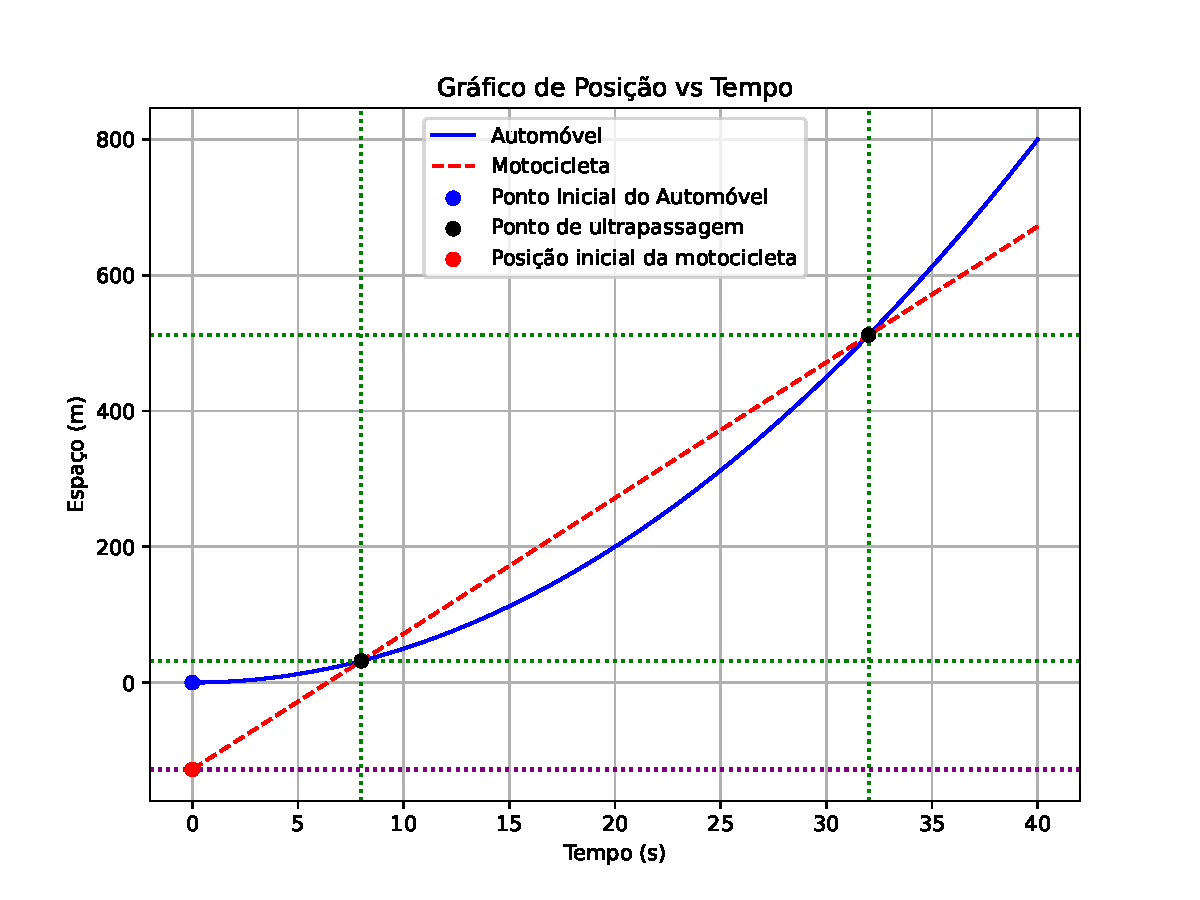
\includegraphics[width=0.9\textwidth]{images/grafico_posicao_tempo.pdf}  % Caminho do arquivo PDF
    \caption{Gráfico de Posição vs Tempo}
    \label{fig:grafico}
\end{figure}

\noindent
\begin{minipage}{0.6\textwidth}
\textbf{12.} Uma luminária cuja massa é de 20 kg precisa ser fixada a uma distância de 1,5 m do teto por meio de três cabos de 2 m (inextensíveis e de massa desprezível), conforme a figura ao lado. Para que seja feita a escolha do material do cabo, faz-se necessário determinar a tensão a que o cabo será submetido.

Sabendo que o valor da aceleração da gravidade no local de instalação da luminária é de \(9,8 \, \mathrm{m/s}^2\), qual o valor da tensão em cada um dos cabos?

\begin{itemize}
    \item[a)] 261,33 N.
    \item[b)] 147 N.
    \item[c)] 87,11 N.
    \item[d)] 49 N.
\end{itemize}
\end{minipage}
\hfill
\begin{minipage}{0.35\textwidth}
\centering
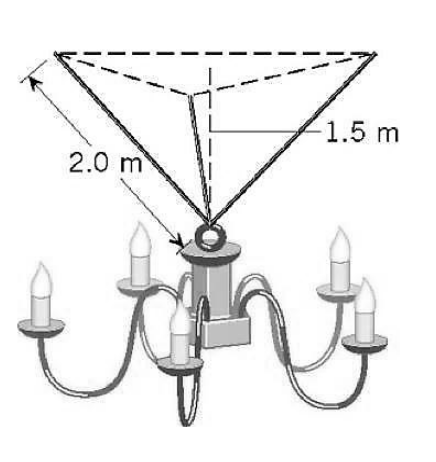
\includegraphics[width=\linewidth]{images/luminaria.png} % substitua pelo nome correto da imagem
\end{minipage}

\section*{Solução}

Passo 1: Determinar o peso da luminária.

\[
P = m \cdot g = 20 \cdot 9,8 = 196 \, \mathrm{N}
\]

Como a luminária é sustentada por três cabos, cada cabo contribui igualmente para sustentar o peso. Assim, a força vertical em cada cabo é:

\[
\frac{196}{3} \approx 65,33 \, \mathrm{N}
\]

\bigskip
Passo 2: Determinar o ângulo formado pelos cabos.

Os cabos possuem comprimento de \(2,0 \, \mathrm{m}\) e a luminária está a \(1,5 \, \mathrm{m}\) do teto. O ângulo de inclinação \(\theta\) pode ser obtido a partir do cosseno:

\newpage
\begin{tikzpicture}
    % Eixos principais (em verde, como no seu exemplo)
    \draw[->,thick,black] (0,0) -- (1,0) node[right] {$x$};
    \draw[->,thick,black] (0,0) -- (0,1) node[above] {$y$};

    % Outro sistema de eixos em azul
    \draw[->,thick,blue] (5,0) -- (7,0);
    \draw[->,thick,blue] (5,0) -- (5,2);

    % Vetor vermelho
    \draw[->,thick,red] (5,0) -- (6,1.5);

    % Ângulo em amarelo
    \draw[thick,black] (5.65,1) arc[start angle=45, end angle=90, radius=0.9];

    % Nome do ângulo
    \node[black] at (5.4,1.5) {$\theta$};

\end{tikzpicture}

\[
\cos \theta = \frac{1,5}{2} = 0,75
\]

\bigskip
Passo 3: Relacionar a componente vertical com a tensão total.

A componente vertical da força em cada cabo é:

\[
T_y = T \cdot \cos \theta
\]

Logo:

\[
65,33 = T \cdot 0,75
\]

\[
T = \frac{65,33}{0,75} \approx 87,11 \, \mathrm{N}
\]

\bigskip
\noindent
Portanto, a tensão em cada cabo é:

\[
\boxed{87,11 \, \mathrm{N}}
\]

\bigskip
\noindent
Alternativa correta: \textbf{(c)}.

%%%%%%%% Bibliography 
% Os comandos para incluir as referências bibliográficas
%\printingbibliography

\end{document}
